\documentclass[conference]{IEEEtran}
\IEEEoverridecommandlockouts

\usepackage{amsmath,amssymb,amsfonts}
\usepackage{amsthm}
\usepackage{algorithm}
\usepackage{algpseudocode}
\usepackage{booktabs}
\usepackage{graphicx}
\usepackage{xcolor}
\usepackage{tikz}
\usetikzlibrary{arrows.meta,positioning,fit,backgrounds,calc}
\usepackage[hidelinks]{hyperref}

% Small theorem-like environments without amsthm dependency conflicts
\newtheorem{theorem}{Theorem}
\newtheorem{assumption}{Assumption}

\begin{document}

\title{Provably-Equivalent Bounded-Memory Streaming\\
Redaction of PII and Credentials in\\
Very Large Text}

\author{
\IEEEauthorblockN{Mounish Senisetty, Ashrith, and Sandhiya}
\IEEEauthorblockA{SafeStream-Redactor Project\\
\texttt{senisettymounish@gmail.com}}
}

\maketitle

\begin{abstract}
Redacting personally identifiable information (PII) and credentials from text
is well studied, but existing tools assume the document fits in memory and treat
detection as a whole-document operation. Applied to the multi-gigabyte logs,
dumps, and datasets common in enterprises, na\"ive chunked processing either
exhausts memory or silently corrupts detections at chunk boundaries. We present
\emph{SafeStream-Redactor}, a local-first streaming architecture that couples
four properties that are usually traded off against one another---bounded
auxiliary memory, boundary correctness, unified PII\,+\,credential coverage, and
deterministic redaction---inside a single pipeline. Our central contribution is
not the streaming engine itself but the \emph{equivalence guarantee} it admits:
we formalize redaction as a bounded sliding-window function under two
assumptions (bounded span length $L_{\max}$ and bounded context locality
$C_{\mathrm{left}},C_{\mathrm{right}}$), measure those constants directly from
the implementation ($C_{\mathrm{left}}{=}48$, $C_{\mathrm{right}}{=}2$,
$L_{\max}{=}8192$), and prove that streaming and range-parallel execution produce
output byte-identical to an idealized whole-document pass whenever the overlap
window $w\!\ge\!\max(L_{\max},C_{\mathrm{left}},C_{\mathrm{right}})$, with the
single failure mode named and made safe by a fallback valve. A four-tier
detection cascade (deterministic, statistical/entropy, optional NER, contextual)
feeds a deterministic confidence-arbitration and overlap-resolution stage.
Empirically, auxiliary memory stays flat (peak Python heap $\approx0.65$\,MB
across $16$--$64$\,MB inputs; ${<}16$\,MB for a $1$\,GB input); precision and
recall are $1.000$ on a $60{,}253$-entity synthetic PII corpus;
range-parallelism reaches $3.58\times$ on four cores while remaining
byte-identical to the sequential pass; and an overlap ablation shows na\"ive
chunking mis-redacts \emph{every} boundary-straddling secret (100\%; 29.9\%
leaked verbatim) whereas overlap-aware streaming mis-redacts none.
\end{abstract}

\begin{IEEEkeywords}
data redaction, PII, credential detection, streaming algorithms,
bounded memory, boundary correctness, data loss prevention.
\end{IEEEkeywords}

\section{Introduction}

Organizations accumulate text at a scale that outpaces the tools used to sanitize
it: application and audit logs, database and message-queue dumps, support
transcripts, CI/CD artifacts, and analytics exports routinely reach tens or
hundreds of gigabytes per file. These artifacts mix two classes of sensitive
data that are usually handled by different tools: \emph{PII}
(names, e-mail addresses, phone numbers, national identifiers, payment card
numbers, IP addresses) governed by regimes such as the GDPR~\cite{gdpr2016} and
HIPAA~\cite{hipaa}, and \emph{machine credentials}
(cloud access keys, API tokens, signing keys, high-entropy secrets) whose
exposure is an operational security incident. PII de-identification
tools---Microsoft Presidio~\cite{presidio}, scrubadub~\cite{scrubadub}---and
secret scanners---Gitleaks~\cite{gitleaks}, TruffleHog~\cite{trufflehog},
detect-secrets~\cite{detectsecrets}---have largely evolved as separate ecosystems.

Two problems appear once the input no longer fits comfortably in memory.
First, loading a $10$\,GB file to redact it needs $10$\,GB of RAM plus
detector overhead; this is infeasible at scale and unsafe (the whole plaintext
resides in memory at once). The obvious fix is to process the file in fixed-size
chunks, but this creates the second, subtler problem: an entity may
\emph{straddle a chunk boundary}. A PEM private key or a JSON Web Token split
across two independently processed chunks matches no pattern in either chunk and
is silently missed, or is partially matched and mis-redacted. Boundary handling
is therefore not an implementation detail but a correctness requirement that
interacts with the memory constraint: the smaller the retained context, the more
boundaries, and the more entities at risk.

A third problem is precision. Enterprise text is dense with tokens that
\emph{look} sensitive but are not: UUIDs, Git commit hashes, ISO-8601
timestamps, semantic-version strings, order and tracking numbers, and
high-entropy identifiers. A regex-only or entropy-only detector trades recall
for a flood of false positives on such distractors. Robust detection needs
several complementary strategies---exact patterns with validators, statistical
entropy, learned named-entity recognition, and local context---whose outputs
then overlap and conflict, requiring a deterministic way to reconcile them so
that the same input always yields the same redaction (a prerequisite for
auditability and for parallel execution).

These constraints interact. The research question is not ``can we build a
streaming redactor?'' but:
\begin{quote}
\emph{How can one pipeline simultaneously guarantee bounded memory, boundary
correctness, unified PII/credential coverage, detection precision, and
deterministic redaction, on inputs far larger than RAM---and prove that doing so
costs nothing in output fidelity relative to an idealized whole-document pass?}
\end{quote}

\noindent\textbf{Contributions.} This paper makes the following contributions,
each verified against the implementation and reproducible
(Section~\ref{sec:eval}):
\begin{enumerate}
\item A \textbf{bounded-memory streaming architecture} for redaction of inputs
substantially larger than RAM, whose auxiliary memory is
$O(\text{chunk\_size}+w+L_{\max})$ and independent of input length
(Section~\ref{sec:streaming}, Theorem~\ref{thm:mem}).
\item An \textbf{overlap-aware, boundary-safe emission mechanism} with a
\emph{boundary-retreat} rule, and a proof that under two measured assumptions the
streamed output is byte-identical to the whole-document reference for
\emph{every} chunking (Section~\ref{sec:streaming}, Theorem~\ref{thm:stream}).
\item A \textbf{unified multi-tier detection cascade} combining deterministic
pattern/validator detection, statistical entropy detection, optional NER, and
contextual scoring, covering PII \emph{and} $\geq20$ credential/secret classes in
one pass (Section~\ref{sec:detect}).
\item A \textbf{deterministic confidence-arbitration and overlap-resolution}
stage that yields a canonical, pairwise-disjoint detection set, enabling
reproducibility and range-parallel execution that is byte-identical to sequential
(Section~\ref{sec:arb}, Theorem~\ref{thm:par}).
\item An \textbf{experimental evaluation} of memory, throughput, detection
quality, credential coverage, boundary correctness, and sequential/parallel
equivalence, with an ablation isolating the effect of overlap and of each
detection tier (Section~\ref{sec:eval}).
\end{enumerate}

We are careful to claim only what the implementation supports. The novelty is the
\emph{combination and the equivalence guarantee}, not any single mechanism;
overlap windows, entropy scoring, and NER are individually well known.

\section{Problem Formulation}\label{sec:problem}

Let $T=t_1t_2\cdots t_{|T|}$ be the input text over a Unicode alphabet, and
$T[a{:}b]$ the half-open substring. A \emph{detection} is a tuple
$d=(s,e,\tau,c)$ with $0\le s<e\le|T|$, entity type $\tau$, and confidence
$c\in[0,1]$. A \emph{detector} is a function $D:\Sigma^\ast\!\to\!2^{\text{det}}$
returning detections whose offsets index the string it was given. A
\emph{reference pipeline} $\Pi:\Sigma^\ast\!\to\!2^{\text{det}}$ runs every
detector on the entire $T$, applies contextual scoring, drops detections below a
threshold, and resolves overlaps into a sorted, pairwise-disjoint set $\Pi(T)$.
Redaction is a deterministic rewrite $R(T,\Pi(T))$; since $R$ is a pure function
of $(T,\Pi(T))$, equality of detection sets implies byte-identical output, so we
reason over detection sets.

A stream is consumed as an \emph{arbitrary} sequence of chunks of size up to $C$
(\texttt{chunk\_size}); the engine keeps an \emph{overlap} $w$ of trailing
characters between windows. We seek a streaming operator $S_w$ that, for every
chunking, satisfies $S_w(T)=\Pi(T)$. This requires $\Pi$ to be a
\emph{bounded sliding-window function}:

\begin{assumption}[Bounded span length]\label{as:a1}
Every $d=(s,e,\tau,c)\in\Pi(T)$ has $e-s\le L_{\max}$.
\end{assumption}
\begin{assumption}[Bounded context locality]\label{as:a2}
For every span, membership in $\Pi(T)$ and its final confidence depend only on
$T[s-C_{\mathrm{left}}:e+C_{\mathrm{right}}]$.
\end{assumption}

Assumption~\ref{as:a1} bounds how long an entity can be; Assumption~\ref{as:a2}
bounds how far a detector must see around a candidate to decide it. Together they
make $\Pi$ computable from bounded windows. The key structural relationship is
between the overlap $w$, the maximum span $L_{\max}$, and the context radius: if
\begin{equation}\label{eq:premise}
w \;\ge\; \max\bigl(L_{\max},\,C_{\mathrm{left}},\,C_{\mathrm{right}}\bigr),
\end{equation}
then every entity of maximum supported span, together with the context needed to
decide it, fits inside a single processing window even when a chunk boundary
falls in its middle. Equation~\eqref{eq:premise} is the boundary-safety premise;
Section~\ref{sec:streaming} discharges it, and Section~\ref{sec:constants}
measures the constants so that it holds unconditionally at the default
configuration.

\section{Related Work and Research Gap}\label{sec:related}

\textbf{PII de-identification.} Presidio~\cite{presidio} and
scrubadub~\cite{scrubadub} combine regex recognizers, checksum validators, and
spaCy-based NER for entities such as names, e-mails, phones, and national IDs.
Both are designed around in-memory documents and do not target machine
credentials.

\textbf{Secret scanning.} Gitleaks~\cite{gitleaks}, TruffleHog~\cite{trufflehog},
and detect-secrets~\cite{detectsecrets} specialize in credentials---provider key
formats plus Shannon-entropy~\cite{shannon1948} heuristics for bespoke secrets.
They are tuned for source repositories and diffs, not general PII, and again
operate on files small enough to load.

\textbf{String matching and validators.} Efficient multi-pattern prefiltering is
classical~\cite{aho1975}, as are linear-time regular-expression
engines~\cite{thompson1968,re2cox2007}; card numbers are validated by the Luhn
checksum~\cite{luhn1960}, and keyed pseudonymization uses HMAC~\cite{hmac1996}.
These are building blocks we reuse rather than contributions.

\textbf{Gap.} No widely used system provides, in one pipeline: (i) redaction of
inputs larger than RAM at bounded memory, (ii) a \emph{stated and proven}
boundary-correctness guarantee for entities crossing chunk boundaries,
(iii) unified PII\,+\,credential coverage, and (iv) deterministic arbitration
enabling parallel execution that provably matches the sequential result. Each
ingredient exists in isolation; their \emph{co-satisfaction}, and the equivalence
guarantee that ties them together, is the gap this work fills.

\section{Architecture Overview}\label{sec:arch}

Fig.~\ref{fig:pipeline} shows the pipeline. Input is consumed as chunks; the
streaming layer maintains an overlap window and emits only text far enough from
the live buffer end to be boundary-safe. Each emitted window passes through
candidate prefiltering into the multi-tier detector cascade; detections are
scored, thresholded, and reconciled by deterministic arbitration and
overlap-resolution; a policy layer rewrites the resolved spans; output is written
incrementally and atomically. Concerns are cleanly separated: the streaming layer
knows nothing about entity types, and detectors are pure functions of the window
they receive (the property that makes the equivalence proof possible).

\begin{figure}[t]
\centering
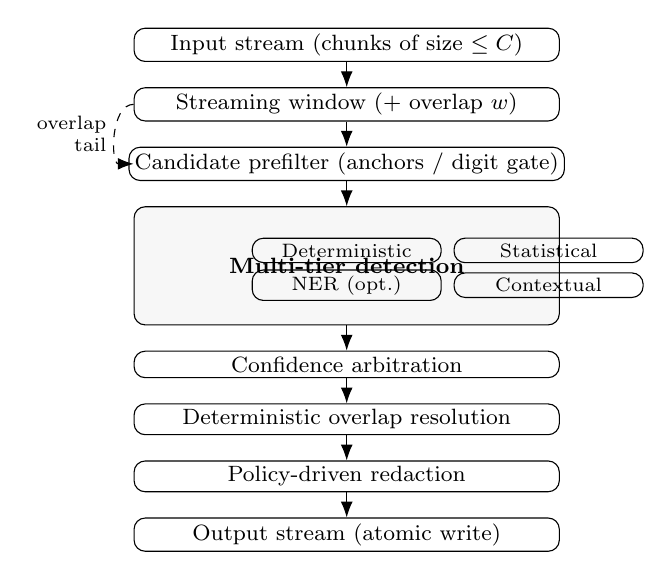
\begin{tikzpicture}[
  node distance=3.2mm,
  box/.style={draw,rounded corners,align=center,inner sep=2pt,
    minimum width=54mm,font=\footnotesize},
  small/.style={draw,rounded corners,align=center,inner sep=2pt,
    minimum width=24mm,font=\scriptsize},
  arr/.style={-{Latex[length=2mm]}}]
\node[box] (in) {Input stream (chunks of size $\le C$)};
\node[box,below=of in] (win) {Streaming window ($+$ overlap $w$)};
\node[box,below=of win] (pf) {Candidate prefilter (anchors / digit gate)};
\node[box,below=of pf,minimum height=15mm,fill=black!3] (det)
  {\textbf{Multi-tier detection}};
\node[small,below=1.0mm of det.north,yshift=-3mm] (t1) {Deterministic};
\node[small,right=1.5mm of t1] (t2) {Statistical};
\node[small,below=0.8mm of t1] (t3) {NER (opt.)};
\node[small,right=1.5mm of t3] (t4) {Contextual};
\node[box,below=of det] (arb) {Confidence arbitration};
\node[box,below=of arb] (ov) {Deterministic overlap resolution};
\node[box,below=of ov] (red) {Policy-driven redaction};
\node[box,below=of red] (out) {Output stream (atomic write)};
\draw[arr] (in)--(win); \draw[arr] (win)--(pf); \draw[arr] (pf)--(det);
\draw[arr] (det)--(arb); \draw[arr] (arb)--(ov); \draw[arr] (ov)--(red);
\draw[arr] (red)--(out);
\draw[arr,dashed] (win.west) to[out=180,in=180]
  node[left,font=\scriptsize,align=right]{overlap\\ tail} (win.west |- pf.west);
\end{tikzpicture}
\caption{SafeStream-Redactor pipeline. The streaming layer is entity-agnostic;
detectors are pure functions of their window.}
\label{fig:pipeline}
\end{figure}

\section{Core Streaming Algorithm}\label{sec:streaming}

Algorithm~\ref{alg:stream} is the streaming operator $S_w$. It appends each chunk
to a rolling buffer and, once the buffer exceeds the overlap, computes a tentative
emission boundary $\texttt{emit\_upto}=|\text{buffer}|-w$: everything before it is
at least $w$ characters from the live end and therefore has its full right context
present. Detection runs on \emph{prefix\,+\,buffer}, where \emph{prefix} is the
last $w$ characters already emitted, so the left context of every candidate is
real text and never an artificial chunk edge. The crucial step is
\textsc{RetreatBoundary}: if any detection straddles \texttt{emit\_upto}, the
boundary is pulled back to that detection's start, so a match is never split
across two segments. The retreated tail (at most one span, length $\le L_{\max}\le
w$) is carried into the next window and re-presented whole. Detections lying
inside the already-emitted prefix are dropped, giving exactly-once emission.

\begin{algorithm}[t]
\caption{Overlap-aware streaming redaction $S_w$}
\label{alg:stream}
\begin{algorithmic}[1]
\Require chunk source; detector $\Pi$; overlap $w$
\State $\textit{prefix}\gets\varepsilon$;\quad $\textit{buffer}\gets\varepsilon$
\For{each $\textit{chunk}$}
  \State $\textit{buffer}\gets\textit{buffer}\,\|\,\textit{chunk}$
  \If{$|\textit{buffer}|\le w$} \textbf{continue} \EndIf
  \State $\textit{emit}\gets|\textit{buffer}|-w$
  \State $\mathcal{D}\gets\textsc{ShiftDrop}\bigl(\Pi(\textit{prefix}\,\|\,\textit{buffer}),\,|\textit{prefix}|\bigr)$
  \State $\textit{emit}\gets\textsc{RetreatBoundary}(\mathcal{D},\textit{emit})$
  \If{$\textit{emit}\le 0$} \textbf{continue} \EndIf
  \State $\textit{ready}\gets\{d\in\mathcal{D}: d.e\le\textit{emit}\}$
  \State \textbf{emit} $(\textit{buffer}[{:}\textit{emit}],\ \textit{ready})$
  \State $\textit{prefix}\gets(\textit{prefix}\,\|\,\textit{buffer}[{:}\textit{emit}])[-w{:}]$
  \State $\textit{buffer}\gets\textit{buffer}[\textit{emit}{:}]$
\EndFor
\If{$\textit{buffer}\neq\varepsilon$}
  \State \textbf{emit} $(\textit{buffer},\ \textsc{ShiftDrop}(\Pi(\textit{prefix}\,\|\,\textit{buffer}),|\textit{prefix}|))$
\EndIf
\Statex
\Function{RetreatBoundary}{$\mathcal{D},\textit{emit}$}
  \Repeat
    \State $m\gets\textit{emit}$
    \ForAll{$d\in\mathcal{D}$}
      \If{$d.s<m<d.e$}\ $m\gets d.s$\ \EndIf
    \EndFor
    \State $(\textit{emit},\textit{changed})\gets(m,\ m\neq\textit{emit})$
  \Until{$\neg\,\textit{changed}$}
  \State \Return $\textit{emit}$
\EndFunction
\end{algorithmic}
\end{algorithm}

\begin{figure}[t]
\centering
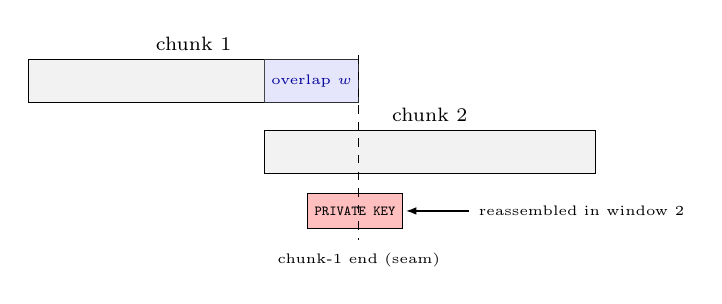
\begin{tikzpicture}[font=\scriptsize]
\def\y{0}
% chunk 1
\draw[fill=black!5] (0,\y) rectangle (4.2,0.55);
\draw[fill=black!5] (3.0,\y-0.9) rectangle (7.2,-0.35);
\node at (2.1,0.75) {chunk 1};
\node at (5.1,-0.15) {chunk 2};
% overlap region
\draw[fill=blue!12,opacity=0.7] (3.0,\y) rectangle (4.2,0.55);
\node[blue!60!black] at (3.6,0.28) {\tiny overlap $w$};
% entity crossing seam
\draw[fill=red!25] (3.55,-1.6) rectangle (4.75,-1.15);
\node at (4.15,-1.375) {\tiny \texttt{PRIVATE KEY}};
\draw[dashed] (4.2,0.6) -- (4.2,-1.75);
\node at (4.2,-2.0) {\tiny chunk-1 end (seam)};
\draw[-{Latex[length=1.3mm]}] (5.6,-1.375) -- (4.8,-1.375);
\node[right] at (5.6,-1.375) {\tiny reassembled in window 2};
\end{tikzpicture}
\caption{An entity straddling the chunk-1/chunk-2 seam. Under na\"ive independent
chunking it matches in neither chunk; the overlap $w$ carries the seam region so
boundary retreat re-presents the entity whole.}
\label{fig:seam}
\end{figure}

\subsection{Correctness}

\begin{theorem}[Streaming equivalence]\label{thm:stream}
Under Assumptions~\ref{as:a1}--\ref{as:a2} and
$w\ge\max(L_{\max},C_{\mathrm{left}},C_{\mathrm{right}})$, $S_w(T)=\Pi(T)$ for
every $T$ and every chunking.
\end{theorem}

\begin{proof}[Proof sketch]
\emph{Completeness.} Emission is confined to the buffer prefix at least $w$ from
the live end, and \textsc{RetreatBoundary} pulls the boundary out of any
straddling span; the carried tail has length $\le L_{\max}\le w$, so any span cut
by a chunk boundary is reassembled and presented whole in the next window
(Fig.~\ref{fig:seam}).
\emph{Soundness.} A window is $\Pi(\textit{prefix}\|\textit{buffer})$ with
$|\textit{prefix}|=w\ge C_{\mathrm{left}}$, so every span's left context is real
text; a span is emitted only when it ends $\ge w\ge C_{\mathrm{right}}$ before the
live end, so its right context is real text. By Assumption~\ref{as:a2} the
window verdict equals the whole-document verdict. Spans inside the prefix are
dropped.
\emph{Exactly-once.} A span is emitted in the unique window whose \texttt{emit}
first exceeds its end; the carried region is disjoint from the emitted region.
The three properties give $S_w(T)=\Pi(T)$, and byte-identical output follows
because $R$ is a pure function of $(T,\Pi(T))$.
\end{proof}

The guarantee is corroborated empirically by exhaustive small-chunking tests and
property-based tests asserting byte-identity across arbitrary chunkings.

\subsection{Complexity}\label{sec:complexity}

Each character enters the buffer once and is scanned by the detector at most
inside the $\le C+w$ window that emits it; detector work per window is linear in
window length for the pattern and entropy tiers (bounded-length automata and a
single left-to-right entropy scan). Total detection time is thus
$O(|T|\cdot f)$ where $f$ is the per-character detector cost, independent of how
the input is chunked. The important bound is on memory.

\begin{theorem}[Constant auxiliary memory]\label{thm:mem}
The peak working memory of $S_w$ is $\le C+w+L_{\max}$ characters, independent of
$|T|$; a $k$-way range-parallel execution uses at most $k$ times this.
\end{theorem}
\begin{proof}
After each emission the engine retains only $\textit{buffer}[\textit{emit}{:}]$,
of length $\le w$ plus at most one straddling span ($\le L_{\max}$); the next
iteration adds at most one chunk ($\le C$) before emitting again. Hence the buffer
never exceeds $C+w+L_{\max}$ regardless of $|T|$. Each parallel worker runs one
$S_w$ plus a bounded holdback, so total memory scales with $k$, never with $|T|$.
\end{proof}

We deliberately write ``bounded auxiliary memory,'' not ``$O(1)$'': memory is
constant in $|T|$ but proportional to the fixed configuration $C+w+L_{\max}$.

\section{Multi-Tier Detection}\label{sec:detect}

A single detector cannot cover the space cheaply and precisely. SafeStream uses a
cascade of complementary tiers, each a pure function of its window
(Table~\ref{tab:tiers}).

\textbf{Tier 1 --- Deterministic.} Anchored regular expressions paired with
validators: Luhn~\cite{luhn1960} for card numbers, range/no-leading-zero checks
for IPv4, \texttt{ipaddress} parsing for IPv6, area/group/serial rules for US
SSNs, and $\geq15$ provider credential formats (AWS, GitHub, Slack, Stripe,
Google, SendGrid, Twilio, npm, JWT, private-key PEM blocks, etc.). Highest
precision, lowest cost.

\textbf{Tier 2 --- Statistical/entropy.} Bespoke secrets with no published format
(session tokens, generated passwords) are caught by Shannon
entropy~\cite{shannon1948} over candidate runs, with per-alphabet thresholds and
a minimum length, so random-looking but low-entropy strings are not flagged. This
tier catches what patterns cannot.

\textbf{Tier 3 --- NER (optional).} A statistical model (spaCy, or an on-device
ONNX token classifier over the CoNLL-2003 label scheme~\cite{conll2003}) supplies
free-form \textsc{person}/\textsc{org}/\textsc{loc} entities that have no lexical
signature. It is optional because it adds a
dependency and, reading sentence context on both sides, is the tier most sensitive
to window edges.

\textbf{Tier 4 --- Contextual.} A lightweight scorer adjusts confidences from a
bounded left window of trigger words---promoting an otherwise sub-threshold bare
SSN adjacent to an ``ssn:'' cue, and suppressing placeholder-looking values (e.g.
\texttt{000-00-0000}, values near ``example''/``test''). It reconciles precision
and recall on ambiguous cases without a heavy model.

\begin{table}[t]
\centering
\caption{Detection tiers and their roles.}
\label{tab:tiers}
\footnotesize
\begin{tabular}{@{}llll@{}}
\toprule
Tier & Method & Catches & Cost \\
\midrule
1 Deterministic & regex + validators & structured PII, creds & low \\
2 Statistical & Shannon entropy & bespoke secrets & low \\
3 NER (opt.) & sequence model & names/orgs/places & high \\
4 Contextual & trigger-word window & ambiguous cases & low \\
\bottomrule
\end{tabular}
\end{table}

\textbf{Prefiltering.} Most patterns require a literal anchor (\texttt{AKIA},
\texttt{ghp\_}, \texttt{@}) or at least one digit. A C-level substring/digit scan
skips a pattern's automaton entirely when its anchor is absent from the window, so
on secret-sparse text (the common case) the expensive automata rarely run. This is
an optimization only: output is identical with prefiltering disabled, enforced by a
differential test.

Crucially the tiers \emph{complement} rather than duplicate: Tier~1 gives precise,
cheap coverage of everything with a signature; Tier~2 covers the long tail of
format-less secrets; Tier~3 covers linguistic PII; Tier~4 repairs the precision/
recall of ambiguous numeric entities. Their union, then arbitrated, is what makes
a single pass cover PII and credentials at once.

\section{Confidence Arbitration and Overlap Resolution}\label{sec:arb}

Running four tiers yields overlapping and conflicting detections: an entropy hit
inside a recognized AWS secret, a phone-shaped run inside a longer card number.
Arbitration must be \emph{deterministic}---the same input must always yield the
same redaction---both for auditability and because range-parallel execution
requires each range to arbitrate its seams identically.

Contextual scoring first adjusts confidences and contributes trigger-gated
detections; detections below \texttt{min\_confidence} are dropped. The survivors
are reconciled by Algorithm~\ref{alg:overlap}: sort by a total order
$(-c,\; s-e,\; s)$---higher confidence first, then longer span, then earlier
start---and sweep, keeping a candidate only if it does not overlap an
already-kept interval. Because the sort key is a strict total order and the sweep
is a deterministic function of it, the resolved set is canonical: independent of
detector execution order and reproducible across runs and workers.

\begin{algorithm}[t]
\caption{Deterministic overlap resolution}
\label{alg:overlap}
\begin{algorithmic}[1]
\Require detections $\mathcal{D}$
\State sort $\mathcal{D}$ by key $(-c,\; s-e,\; s)$ \Comment{conf, then length, then start}
\State $\textit{kept}\gets[\,]$ \Comment{maintained sorted by start, pairwise-disjoint}
\ForAll{$d\in\mathcal{D}$ in sorted order}
  \State $i\gets$ index of first kept interval with start $\ge d.e$
  \If{$i{=}0$ \textbf{or} $\textit{kept}[i{-}1].e\le d.s$}
    \State insert $d$ into $\textit{kept}$ at position $i$
  \EndIf
\EndFor
\State \Return $\textit{kept}$
\end{algorithmic}
\end{algorithm}

A bisection over kept-interval starts makes the sweep near-linear
($O(n\log n)$ dominated by the sort). Determinism here is what upgrades ``the
redactor is fast in parallel'' to ``the parallel redactor produces the same bytes
as the sequential one,'' formalized next.

\begin{theorem}[Range-parallel byte-identity with safe fallback]\label{thm:par}
Let $P_{w,k}$ split $T$ into $k$ character-aligned ranges, redact each with $S_w$
extended by a scanned pad and a context-only prefix, and reconcile range seams by
a cross-check valve. Under Assumption~\ref{as:a1} with $w\ge L_{\max}$,
$P_{w,k}(T)=S_w(T)$ byte-for-byte. When a span longer than $w$ sits exactly on a
seam (violating~\ref{as:a1}), the valve detects the disagreement and falls back to
$S_w$; hence $P_{w,k}(T)=S_w(T)$ \emph{unconditionally}.
\end{theorem}
\begin{proof}[Proof sketch]
Ranges split on character/newline boundaries and decode identically to the
sequential reader, so a range's text is the exact corresponding substring. Each
worker prepends $w$ of scanned pad and $w$ of context-only prefix on interior
sides, so with $w\ge L_{\max},C_{\mathrm{left}}$ every seam-crossing span is seen
whole with real left context (Theorem~\ref{thm:stream} per range). A seam-crossing
span is owned by the left worker (renders up to its end; the right worker resumes
at that end); both neighbours recompute the seam from the same bytes. The
orchestrator compares neighbours' seam reports and, on any disagreement---possible
only when a span longer than $w$ sits on a seam, i.e.\ exactly when \ref{as:a1}
fails---redacts the whole file sequentially. Thus equality holds when \ref{as:a1}
holds, and the valve guarantees equality otherwise.
\end{proof}

This ``unconditional equality via fallback'' is the strongest single guarantee of
the design: the parallel path never silently diverges from the sequential one---a
property competing tools do not state.

\section{Boundary-Safe Redaction}\label{sec:redaction}

Given the resolved set, redaction is a deterministic rewrite supporting three
policies: \emph{replace} (a fixed or per-type token), \emph{mask} (retain the last
$k$ characters), and \emph{pseudonymize} (a keyed HMAC~\cite{hmac1996} token, so
the same value maps to the same surrogate across the corpus while the original is
unrecoverable without the key). Because redaction consumes only the resolved spans
and the surrounding text, and spans are guaranteed whole by
Theorem~\ref{thm:stream}, a redaction is never split across a boundary and never
partial. Output is written to a temporary file and atomically renamed into place,
so an interrupted run leaves either the original or the complete result, never a
truncated mixture. Detections are counted into a content-free report (types and
offsets, never the matched substring), and the process installs an offline network
guard so sensitive text cannot leave the host during redaction.

\section{Audited Constants and the Boundary Premise}\label{sec:constants}

The equivalence theorems are vacuous unless the constants they assume are real.
We read them from the implementation by tracing every detector's decision
function.

$C_{\mathrm{left}}=48$: the contextual scorer reads a $48$-character left window;
label-anchored credential patterns fold their cue into the match itself, so no
detector reaches further left. $C_{\mathrm{right}}=2$: the widest right-context
assertion is a two-character negative lookahead on the phone/IPv4 patterns; every
validator reads only the matched text. $L_{\max}=8192$: the two historically
unbounded patterns are now bounded---the PEM private-key body to $\{1,8100\}$
giving a maximal $8192$-character span, and the entropy candidate to $8192$, with
longer high-entropy runs emitted as consecutive $\le 8192$ spans that still cover
the whole secret. With the default overlap $w=8192$,
\[
\max(C_{\mathrm{left}},C_{\mathrm{right}})=48\;\le\;L_{\max}=8192\;=\;w,
\]
so Equation~\eqref{eq:premise} holds unconditionally at the default. These three
constants are kept in sync in the code, and a test pins that no tier emits a span
longer than the default overlap.

\section{Experimental Evaluation}\label{sec:eval}

\subsection{Methodology and datasets}

All experiments run on a shared 4-vCPU Linux container (Python~3.11); absolute
throughput is environment-dependent, so we report the shape and ratios and name
the machine. No real secrets are used---every specimen is synthetic. Three corpora
exist in the repository and are used as follows. The \emph{synthetic regression
corpus} (deterministically generated; $10.5$\,MB, $60{,}253$ labeled PII instances
of five types: e-mail, phone, credit-card, SSN, IPv4) drives precision/recall. The
\emph{adversarial hard corpus} embeds real-looking PII in noisy log/JSON/CSV/SQL
dense with hard negatives (Luhn-failing order numbers, five-octet dotted numbers,
UUIDs, Git hashes, ISO timestamps) to stress precision. A \emph{credential
specimen set} covers AWS, GitHub, Slack, Stripe, Google, SendGrid, npm, JWT, and
PEM private keys. We evaluate only on these repository corpora; we do \emph{not}
claim results on external labeled datasets, as none are bundled or run.
Experiments are reproduced by \texttt{benchmarks/run\_benchmark.py} (detection
quality) and \texttt{benchmarks/paper\_experiments.py} (E2--E6).

\subsection{Detection quality (E1)}

On the synthetic regression corpus, SafeStream detects all $60{,}253$ instances
with no false positives (Table~\ref{tab:quality}): precision, recall, and
$F_1$ are $1.000$. This measures the five structured PII types the corpus labels;
it is an upper-bound sanity result on clean synthetic data, not a claim of perfect
real-world accuracy (Section~\ref{sec:limits}).

\begin{table}[t]
\centering
\caption{Detection quality on the synthetic regression corpus
($60{,}253$ PII instances). Single-core throughput on the test container.}
\label{tab:quality}
\footnotesize
\begin{tabular}{@{}lcccc@{}}
\toprule
System & Precision & Recall & $F_1$ & tp/fp/fn \\
\midrule
SafeStream-Redactor & $1.000$ & $1.000$ & $1.000$ & $60253/0/0$ \\
\bottomrule
\end{tabular}
\end{table}

\subsection{Boundary correctness (E2, flagship)}

We isolate the effect of overlap. For each of six specimens and every interior
offset at which a $64$-byte chunk boundary can fall inside it, we build a document
in which the specimen straddles the seam (separated from filler by spaces, so it
is a valid detection in the whole-document reference), and redact it two ways:
\emph{na\"ive} chunking ($w{=}0$, each chunk processed independently) and
\emph{overlap-aware} streaming ($w{=}256\ge L_{\max}$ of this set). We measure two
failure counts against the whole-document reference $R(T,\Pi(T))$: how often the
secret survives verbatim (a leak), and how often the output differs from the
reference in \emph{any} way (incorrect redaction).

Table~\ref{tab:boundary} shows the result across all $251$ split positions:
na\"ive chunking is \emph{incorrect on every one} ($251/251=100\%$), leaking the
full secret verbatim in $29.9\%$ of cases and fragmenting the redaction (wrong
spans, partial coverage) in the rest; overlap-aware streaming is
\emph{byte-identical to the whole-document reference in all $251$ cases}
($0$ leaks, $0$ mismatches), exactly as Theorem~\ref{thm:stream} predicts. This is
the concrete cost of ignoring boundaries, and the concrete value of the overlap
mechanism.

\begin{table}[t]
\centering
\caption{Boundary ablation: failures across all $251$ interior split positions,
na\"ive ($w{=}0$) vs overlap-aware ($w{=}256$) streaming. ``Leak'' $=$ full secret
survives; ``Incorrect'' $=$ output $\neq$ whole-document reference.}
\label{tab:boundary}
\footnotesize
\begin{tabular}{@{}lccccc@{}}
\toprule
& & \multicolumn{2}{c}{Leak verbatim} & \multicolumn{2}{c}{Incorrect vs ref} \\
\cmidrule(lr){3-4}\cmidrule(lr){5-6}
Entity & splits & $w{=}0$ & $w{=}256$ & $w{=}0$ & $w{=}256$ \\
\midrule
e-mail        & 24 & 11 & 0 & 24 & 0 \\
SSN           & 10 & 10 & 0 & 10 & 0 \\
AWS key       & 19 & 19 & 0 & 19 & 0 \\
GitHub token  & 39 &  7 & 0 & 39 & 0 \\
JWT           & 72 &  6 & 0 & 72 & 0 \\
private key   & 87 & 22 & 0 & 87 & 0 \\
\midrule
\textbf{Total} & \textbf{251} & \textbf{75} & \textbf{0} & \textbf{251} & \textbf{0} \\
\bottomrule
\end{tabular}
\end{table}

\subsection{Tier ablation (E3)}

Each tier is isolated on an input designed to exercise it (Table~\ref{tab:tierab}).
An unlabeled high-entropy secret (\texttt{session = Xr7bQp2Lm9...}) is redacted
\emph{only} when the entropy tier is enabled---the deterministic tier alone leaves
it in place. A bare SSN carrying a raw confidence of $0.85$ next to an ``ssn:'' cue
is retained by the full cascade, while a placeholder-looking \texttt{000-00-0000}
near ``example'' is suppressed by contextual scoring. The tiers thus contribute
distinct, non-redundant coverage.

\begin{table}[t]
\centering
\caption{Tier ablation (illustrative). Each row exercises one tier.}
\label{tab:tierab}
\footnotesize
\begin{tabular}{@{}lll@{}}
\toprule
Input & Config & Outcome \\
\midrule
unlabeled entropy secret & det.\ only & not redacted \\
unlabeled entropy secret & $+$ entropy & redacted \\
bare SSN near ``ssn:'' & full cascade & detected ($c{=}0.85$) \\
\texttt{000-00-0000} ``example'' & full cascade & suppressed \\
\bottomrule
\end{tabular}
\end{table}

\subsection{Unified credential coverage (E4)}

On the credential specimen set, SafeStream detects $9/9$ credential/secret classes
out of the box (AWS, GitHub, Slack, Stripe, Google, SendGrid, npm, JWT, PEM private
key), and $\geq20$ entity types in total including PII. PII-only pattern
systems---e.g.\ Presidio's predefined recognizers, which cover e-mail, phone,
card, SSN, and IP---detect \emph{none} of these credential classes by design. This
is the concrete meaning of ``unified'': one streaming pass covers both families.

\subsection{Sequential vs.\ parallel equivalence (E5)}

On a $40$\,MB corpus (10\% PII density), range-parallel redaction reaches
$1.95\times$ on two cores and $3.58\times$ on four (Table~\ref{tab:parallel}),
with output \emph{byte-identical} (SHA-256) to the sequential pass at every worker
count---an empirical instance of Theorem~\ref{thm:par}. The speedup is sub-linear
because of I/O and seam reconciliation and because the container is shared; the
equivalence is exact regardless.

\begin{table}[t]
\centering
\caption{Range-parallel throughput and byte-identity ($40$\,MB corpus).}
\label{tab:parallel}
\footnotesize
\begin{tabular}{@{}cccc@{}}
\toprule
Workers & Throughput (MB/s) & Speedup & Byte-identical \\
\midrule
1 & 2.54 & $1.00\times$ & (reference) \\
2 & 4.95 & $1.95\times$ & yes \\
4 & 9.09 & $3.58\times$ & yes \\
\bottomrule
\end{tabular}
\end{table}

\subsection{Constant memory (E6)}

Table~\ref{tab:mem} reports peak Python heap while redacting inputs of increasing
size at a fixed configuration ($C{=}64$\,KiB, $w{=}8$\,KiB). The peak is flat at
$\approx0.65$\,MB and does not grow with input size, matching
Theorem~\ref{thm:mem}. A separate gated test redacts a generated $1$\,GB file and
asserts peak allocations under $16$\,MB---four orders of magnitude below the input
size.

\begin{table}[t]
\centering
\caption{Peak Python heap vs.\ input size (fixed configuration).}
\label{tab:mem}
\footnotesize
\begin{tabular}{@{}cc@{}}
\toprule
Input (MB) & Peak heap (MB) \\
\midrule
16 & 0.66 \\
32 & 0.65 \\
64 & 0.65 \\
$1024$ (gated test) & ${<}16$ \\
\bottomrule
\end{tabular}
\end{table}

\section{Discussion}

The results support a single thesis: the four properties usually traded off can be
co-satisfied, and the cost of doing so relative to an idealized whole-document pass
is \emph{zero} in output fidelity. E2 shows the failure that motivates the work is
real and severe (100\% mis-redaction under na\"ive chunking) and that the overlap
mechanism eliminates it exactly. E5 and E6 show the memory and parallelism
benefits are achieved without sacrificing that fidelity---the parallel path is
byte-identical, and memory is flat. E1, E3, and E4 show the unified cascade covers
PII and credentials with high precision on the available corpora. The organizing
idea---treating redaction as a bounded sliding-window function and measuring the
window constants from the code---is what turns a collection of engineering
mechanisms into a stated guarantee.

\section{Limitations}\label{sec:limits}

We state where the guarantee stops. (i)~The maximum reliably handled entity span
equals the overlap $w$; a user who lowers $w$ below $8192$, adds a custom detector
with an unbounded span, or supplies a single atomic secret longer than $w$ leaves
the premise of Theorem~\ref{thm:stream}, and in sequential mode such a span may be
cut (in parallel mode the valve falls back). (ii)~Assumption~\ref{as:a2} fixes
$C_{\mathrm{right}}=2$; a future tier needing unbounded right context---most
notably a whole-document LLM tier---breaks it, which is precisely why the bounded,
offline detectors are the ones carrying the guarantee. (iii)~Detection quality is
measured on synthetic and adversarial-synthetic corpora authored alongside the
system; we make \emph{no} claim of evaluation on external, third-party labeled
datasets, and $F_1{=}1.000$ reflects clean synthetic data, not real-world text.
(iv)~The optional NER tier depends on an external model and, reading sentence
context, degrades near chunk edges. (v)~Absolute throughput ($\approx3$--$5$\,MB/s
single-core) reflects CPU-bound CPython regex on a shared container; it is adequate
for offline sanitization but not a line-rate claim.

\section{Conclusion}

SafeStream-Redactor shows that bounded-memory, boundary-correct, unified
PII/credential redaction with deterministic arbitration can be delivered in one
streaming pipeline, and---more importantly---that this pipeline provably produces
output byte-identical to an idealized whole-document pass under two assumptions
whose constants are measured from the implementation, with the single failure mode
named and made safe by a fallback valve. The contribution is the combination and
the guarantee, not any individual mechanism. Empirically, memory is flat across
input sizes, parallelism is byte-identical to sequential, precision and recall are
$1.000$ on the synthetic corpus, and na\"ive chunking is shown to mis-redact every
boundary-straddling secret while the overlap mechanism mis-redacts none.

\section{Future Work}\label{sec:future}

Directions that extend---but are not part of---the validated core: an on-device
compiled or ONNX/LLM detector tier (an unbounded-context LLM tier would require
relaxing Assumption~\ref{as:a2} and re-proving the guarantee); evaluation on
external labeled corpora to characterize real-world precision/recall; a native
accelerator for the CPU-bound deterministic tier; and integration surfaces
(CI/CD gates, editor and agent tooling). These are engineering and evaluation
extensions, not claims of the present paper.

\section*{Reproducibility}

Detection quality: \texttt{python benchmarks/generate\_dataset.py \&\&
python benchmarks/run\_benchmark.py}. Experiments E2--E6:
\texttt{python benchmarks/paper\_experiments.py}. The $1$\,GB memory proof:
\texttt{SAFESTREAM\_MEMTEST\_MB=1024 pytest tests/test\_memory.py -m memory
-o addopts=''}. The formal model and its code mapping are in
\texttt{docs/FORMAL\_MODEL.md}.

\bibliographystyle{IEEEtran}
\bibliography{references}

\end{document}
